\documentclass[oneside,authoryear,spanish,a4paper]{ezthesis}
%\documentclass[oneside,authoryear,draft,spanish]{ezthesis}
%\documentclass[oneside,authoryear,draftmarks,spanish]{ezthesis}
%% # Opciones disponibles para el documento #
%%
%% Las opciones con un (*) son las opciones predeterminadas.
%%
%% Modo de compilar:
%%   draft            - borrador con marcas de fecha y sin im'agenes
%%   draftmarks       - borrador con marcas de fecha y con im'agenes
%%   final (*)        - version final de la tesis
%%
%% Tama'no de papel:
%%   letterpaper (*)  - tama'no carta (Am'erica)
%%   a4paper          - tama'no A4    (Europa)
%%
%% Formato de impresi'on:
%%   oneside          - hojas impresas por un solo lado
%%   twoside (*)      - hijas impresas por ambos lados
%%
%% Tama'no de letra:
%%   10pt, 11pt, o 12pt (*)
%%
%% Espaciado entre renglones:
%%   singlespace      - espacio sencillo
%%   onehalfspace (*) - espacio de 1.5
%%   doublespace      - a doble espacio
%%
%% Formato de las referencias bibliogr'aficas:
%%   numbers          - numeradas, p.e. [1]
%%   authoryear (*)   - por autor y a'no, p.e. (Newton, 1997)
%%
%% Opciones adicionales:
%%   spanish         - tesis escrita en espa'nol
%%
%% Desactivar opciones especiales:
%%   nobibtoc   - no incluir la bibiolgraf'ia en el 'Indice general
%%   nofancyhdr - no incluir "fancyhdr" para producir los encabezados
%%   nocolors   - no incluir "xcolor" para producir ligas con colores
%%   nographicx - no incluir "graphicx" para insertar gr'aficos
%%   nonatbib   - no incluir "natbib" para administrar la bibliograf'ia

%% Paquetes adicionales requeridos se pueden agregar tambi'en aqu'i.
%% Por ejemplo:
\usepackage{subfig}
\usepackage{multirow}
\usepackage[activeacute,spanish]{babel}
\usepackage[utf8]{inputenc}
\usepackage{amsmath}
\usepackage{mathtools}
\usepackage{amsmath,amssymb,amsfonts,latexsym,cancel}
\usepackage{rawfonts}
\usepackage{pictexwd}
\usepackage{float}
\usepackage{booktabs}
\usepackage{graphicx}
\numberwithin{equation}{section}
%paquete para diagramas
\usepackage[all]{xy}
\usepackage{mathrsfs}
\usepackage{tikz}
\usetikzlibrary{3d}
%\usepackage{tikz-3dplot}
\usepackage[thinlines]{easytable}
\usepackage[none]{hyphenat}

%Configuracion codigo c++
\usepackage{listings}
\usepackage[T1]{fontenc}
\usepackage{times}
\usepackage{color}
\definecolor{lightblue}{rgb}{0, 0.7, .7}
\definecolor{gray97}{gray}{.97}
\definecolor{gray75}{gray}{.75}
\definecolor{gray45}{gray}{.45}
\lstset{ frame=Ltb,
framerule=0pt,
aboveskip=0.5cm,
framextopmargin=3pt,
framexbottommargin=3pt,
framexleftmargin=0.4cm,
framesep=0pt,
rulesep=.4pt,
backgroundcolor=\color{gray97},
rulesepcolor=\color{black},
%
stringstyle=\ttfamily,
showstringspaces = false,
basicstyle=\tiny\ttfamily,
commentstyle=\color{gray45},
keywordstyle=\bfseries,
%
numbers=left,
numbersep=15pt,
numberstyle=\tiny,
numberfirstline = false,
breaklines=true,
}
% minimizar fragmentado de listados
\lstnewenvironment{listing}[1][]
{\lstset{#1}\pagebreak[0]}{\pagebreak[0]}

\lstdefinestyle{consola}
{basicstyle=\scriptsize\bf\ttfamily,
backgroundcolor=\color{gray75},
}

\lstdefinestyle{C}
{language=C,
}

\lstdefinestyle{customc}{
  belowcaptionskip=1\baselineskip,
  breaklines=true,
  frame=L,
  xleftmargin=\parindent,
  language=C,
  showstringspaces=false,
  basicstyle=\footnotesize\ttfamily,
  keywordstyle=\bfseries\color{green!40!black},
  commentstyle=\itshape\color{purple!40!black},
  identifierstyle=\color{blue},
  stringstyle=\color{orange},
}

\lstdefinestyle{customasm}{
  belowcaptionskip=1\baselineskip,
  frame=L,
  xleftmargin=\parindent,
  language=[x86masm]Assembler,
  basicstyle=\footnotesize\ttfamily,
  commentstyle=\itshape\color{purple!40!black},
}

\lstset{escapechar=@,style=customc,basicstyle=\small}
%



%%##################################################################################################################################
%% # Datos del documento #
%% Nota que los acentos se deben escribir: \'a, \'e, \'i, etc.
%% La letra n con tilde es: \~n.

\author{Pablo Andrés Cárdenas Zamorano}
%\title{SIMULACIÓN DE LAS ESCALAS TURBULENTAS PRINCIPALES DE UNA MEZCLA BIF\'ASICA AGUA-PETROLEO AL INTERIOR DE UN INYECTOR DE TURBINA A GAS MEDIANTE LOS MÉTODO LARGE-EDDY SIMULATION Y VOLUME OF FLUID}
\title{``TÍTULO MUY MUY PRETENCIOSO SOBRE VIENTO EN TERRENO COMPLEJO CON LARGE EDDY SIMULATION Y APLICANDO DATA ASSIMILATION''}
\degree{Magíster en Ciencias de la Ingeniería Mecánica}
\supervisor{Dr. Ing. Alex Flores}
\correferent{Dr. Ing. Olivier Skurtys}
\correferentextern{Dr. Ing. Juan Carlos Elicer}
\institution{UNIVERSIDAD TÉCNICA FEDERICO SANTA MARÍA}
\faculty{Escuela de Ingeniería y Ciencias}
\department{DEPARTAMENTO DE INGENIRIA MECÁNICA}
\city{VALPARAISO}
\country{CHILE}

%% # M'argenes del documento #
%% 
%% Quitar el comentario en la siguiente linea para austar los m'argenes del
%% documento. Leer la documentaci'on de "geometry" para m'as informaci'on.

\geometry{top=40mm,bottom=33mm,inner=40mm,outer=25mm}

%% El siguiente comando agrega ligas activas en el documento para las
%% referencias cruzadas y citas bibliogr'aficas. Tiene que ser *la 'ultima*
%% instrucci'on antes de \begin{document}.
\hyperlinking
\begin{document}

\sloppy 


%% En esta secci'on se describe la estructura del documento de la tesis.
%% Consulta los reglamentos de tu universidad para determinar el orden
%% y la cantidad de secciones que debes de incluir.

%% # Portada de la tesis #
%%% ## Construye tu propia portada ##
%% 
%% Una portada se conforma por una secuencia de "Blocks" que incluyen
%% piezas individuales de informaci'on. Un "Block" puede incluir, por
%% ejemplo, el t'itulo del documento, una im'agen (logotipo de la universidad),
%% el nombre del autor, nombre del supervisor, u cualquier otra pieza de
%% informaci'on.
%%
%% Cada "Block" aparece centrado horizontalmente en la p'agina y,
%% verticalmente, todos los "Blocks" se distruyen de manera uniforme 
%% a lo largo de p'agina.
%%
%% Nota tambi'en que, dentro de un mismo "Block" se pueden cortar
%% lineas usando el comando \\
%%
%% El tama'no del texto dentro de un "Block" se puede modificar usando uno de
%% los comandos:
%%   \small      \LARGE
%%   \large      \huge
%%   \Large      \Huge
%%
%% Y el tipo de letra se puede modificar usando:
%%   \bfseries - negritas
%%   \itshape  - it'alicas
%%   \scshape  - small caps
%%   \slshape  - slanted
%%   \sffamily - sans serif
%%
%% Para producir plantillas generales, la informaci'on que ha sido inclu'ida
%% en el archivo principal "tesis.tex" se puede accesar aqu'i usando:
%%   \insertauthor
%%   \inserttitle
%%   \insertsupervisor
%%	 \insertcorreferent
%%   \insertinstitution
%%   \insertdegree
%%   \insertfaculty
%%   \insertdepartment
%%	 \insertcity
%%	 \insertcountry
%%   \insertsubmitdate

\begin{titlepage}
	\TitleBlock[\vspace{-1.5 in}]{
\includegraphics[height=4cm]{Imagenes/utfsm_logo}}
	\TitleBlock[\vspace{0.05in}]{\bfseries\insertinstitution}
	\TitleBlock[\vspace{0.05in}]{\insertdepartment}
	\TitleBlock[\vspace{0.05in}]{\insertcity  - \insertcountry}
	\TitleBlock[\vspace{1.2in}]{\Large\scshape\bfseries\inserttitle}
    \TitleBlock[\vspace{1.5in}]{\bfseries\insertauthor}
	\TitleBlock[\vspace{0.1in}]{\insertdegree}
	\TitleBlock[\vspace{0.1in}]{Agosto - \insertsubmitdate}
\end{titlepage}

%% Nota 1:
%% Se puede agregar un escudo o logotipo en un "Block" como:
%%   \TitleBlock{\includegraphics[height=4cm]{escudo_uni}}
%% y teniendo un archivo "escudo_uni.pdf", "escudo_uni.png" o "escudo_uni.jpg"
%% en alg'un lugar donde LaTeX lo pueda encontrar.

%% Nota 2:
%% Normalmente, el espacio entre "Blocks" se extiende de modo que el
%% contenido se reparte uniformemente sobre toda la p'agina. Este
%% comportamiento se puede modificar para mantener fijo, por ejemplo, el
%% espacio entre un par de "Blocks". Escribiendo:
%%   \TitleBlock{Bloque 1}
%%   \TitleBlock[\bigskip]{Bloque2}
%% se deja un espacio "grande" y de tama~no fijo entre el bloque 1 y 2.
%% Adem'as de \bigskip est'an tambi'en \smallskip y \medskip. Si necesitas
%% aun m'as control puedes usar tambi'en, por ejemplo, \vspace*{2cm}.



%%%Pagina en blanco sin numeracion
\newpage
$\ $\\
\thispagestyle{empty}
%%% ## Construye tu propia portada ##
%% 
%% Una portada se conforma por una secuencia de "Blocks" que incluyen
%% piezas individuales de informaci'on. Un "Block" puede incluir, por
%% ejemplo, el t'itulo del documento, una im'agen (logotipo de la universidad),
%% el nombre del autor, nombre del supervisor, u cualquier otra pieza de
%% informaci'on.
%%
%% Cada "Block" aparece centrado horizontalmente en la p'agina y,
%% verticalmente, todos los "Blocks" se distruyen de manera uniforme 
%% a lo largo de p'agina.
%%
%% Nota tambi'en que, dentro de un mismo "Block" se pueden cortar
%% lineas usando el comando \\
%%
%% El tama'no del texto dentro de un "Block" se puede modificar usando uno de
%% los comandos:
%%   \small      \LARGE
%%   \large      \huge
%%   \Large      \Huge
%%
%% Y el tipo de letra se puede modificar usando:
%%   \bfseries - negritas
%%   \itshape  - it'alicas
%%   \scshape  - small caps
%%   \slshape  - slanted
%%   \sffamily - sans serif
%%
%% Para producir plantillas generales, la informaci'on que ha sido inclu'ida
%% en el archivo principal "tesis.tex" se puede accesar aqu'i usando:
%%   \insertauthor
%%   \inserttitle
%%   \insertsupervisor
%%	 \insertcorreferent
%%   \insertinstitution
%%   \insertdegree
%%   \insertfaculty
%%   \insertdepartment
%%	 \insertcity
%%	 \insertcountry
%%   \insertsubmitdate

\begin{titlepage}
	\TitleBlock[\vspace{-1.5 in}]{
\includegraphics[height=4cm]{Imagenes/utfsm_logo}}
	\TitleBlock[\vspace{-0.05in}]{
		\bfseries\insertinstitution}
	\TitleBlock[\vspace{-0.05in}]{
		\insertdepartment}
	\TitleBlock[\vspace{-0.05in}]{
		\insertcity - \insertcountry}
	\TitleBlock[\vspace{0.5in}]{
		\small\scshape\bfseries\inserttitle}
	\TitleBlock[\vspace{0.5in}]{
		\small\scshape\bfseries\insertauthor}
    \TitleBlock[\vspace{0.5in}]{
    	Tesis de grado para optar al grado de: \\
    	\textbf{\insertdegree}\\
	    y al titulo de:\\
	    \textbf{Ingeniero Civil Mecánico}}
		\begin{minipage}{0.99\textwidth}
			\TitleBlock[\vspace{0.5in}]{
				\begin{center}
					Profesor Guia: \insertsupervisor
				\end{center}}\vspace{-9mm}
			\TitleBlock{
				\begin{center}
					Profesor Correferente: \insertcorreferent
				\end{center}}\vspace{-9mm}
			\TitleBlock{
				\begin{center}
					Evaluador Externo: \insertcorreferentextern
			\end{center}}
		\end{minipage}
		\TitleBlock{Septiembre - \insertsubmitdate}
\end{titlepage}

%% Nota 1
%% Se puede agregar un escudo o logotipo en un "Block" como:
%%   \TitleBlock{\includegraphics[height=4cm]{escudo_uni}}
%% y teniendo un archivo "escudo_uni.pdf", "escudo_uni.png" o "escudo_uni.jpg"
%% en alg'un lugar donde LaTeX lo pueda encontrar.

%% Nota 2:
%% Normalmente, el espacio entre "Blocks" se extiende de modo que el
%% contenido se reparte uniformemente sobre toda la p'agina. Este
%% comportamiento se puede modificar para mantener fijo, por ejemplo, el
%% espacio entre un par de "Blocks". Escribiendo:
%%   \TitleBlock{Bloque 1}
%%   \TitleBlock[\bigskip]{Bloque2}
%% se deja un espacio "grande" y de tama~no fijo entre el bloque 1 y 2.
%% Adem'as de \bigskip est'an tambi'en \smallskip y \medskip. Si necesitas
%% aun m'as control puedes usar tambi'en, por ejemplo, \vspace*{2cm}.



%%%Pagina en blanco sin numeracion
\newpage
$\ $\\
\thispagestyle{empty}
%%% ## Construye tu propia portada ##
%% 
%% Una portada se conforma por una secuencia de "Blocks" que incluyen
%% piezas individuales de informaci'on. Un "Block" puede incluir, por
%% ejemplo, el t'itulo del documento, una im'agen (logotipo de la universidad),
%% el nombre del autor, nombre del supervisor, u cualquier otra pieza de
%% informaci'on.
%%
%% Cada "Block" aparece centrado horizontalmente en la p'agina y,
%% verticalmente, todos los "Blocks" se distruyen de manera uniforme 
%% a lo largo de p'agina.
%%
%% Nota tambi'en que, dentro de un mismo "Block" se pueden cortar
%% lineas usando el comando \\
%%
%% El tama'no del texto dentro de un "Block" se puede modificar usando uno de
%% los comandos:
%%   \small      \LARGE
%%   \large      \huge
%%   \Large      \Huge
%%
%% Y el tipo de letra se puede modificar usando:
%%   \bfseries - negritas
%%   \itshape  - it'alicas
%%   \scshape  - small caps
%%   \slshape  - slanted
%%   \sffamily - sans serif
%%
%% Para producir plantillas generales, la informaci'on que ha sido inclu'ida
%% en el archivo principal "tesis.tex" se puede accesar aqu'i usando:
%%   \insertauthor
%%   \inserttitle
%%   \insertsupervisor
%%	 \insertcorreferent
%%   \insertinstitution
%%   \insertdegree
%%   \insertfaculty
%%   \insertdepartment
%%	 \insertcity
%%	 \insertcountry
%%   \insertsubmitdate

\begin{titlepage}
	\TitleBlock[\vspace{-1.50in}]{
		\begin{flushleft}
			\small \scshape TÍTULO DE LA TESIS:
		\end{flushleft}
		}
	\TitleBlock[\vspace{0.00in}]{
		\small \textbf{Simulación multiescala del viento sobre terreno complejo mediante el método embebido WRF-LES y asimilación variacional de datos 4D }
		}
	\TitleBlock[\vspace{0.00in}]{
		\begin{flushleft}
			\small AUTOR:
		\end{flushleft}
		}
	\TitleBlock[\vspace{0.0in}]{
		\textbf{\insertauthor}
		}
    \TitleBlock[\vspace{1.0in}]{
    	\small TRABAJO DE TESIS, presentado en cumplimiento parcial de los requisitos para el Grado de \insertdegree de la Universidad T\'ecnica Federico Santa Mar\'ia.
		}
	\begin{minipage}{0.45\textwidth}
		\TitleBlock[\vspace{1in}]{
			\begin{center}
				\small \insertsupervisor
			\end{center}
			}
		\TitleBlock[\vspace{0.3in}]{
			\begin{center}
				\small \insertcorreferent
			\end{center}
			}
		\TitleBlock[\vspace{0.3in}]{
			\begin{center}
				\small \insertcorreferentextern
			\end{center}
		}
	\end{minipage}
	\begin{minipage}{0.45\textwidth}
%		\begin{figure}[H]
%			\centering
%			\vspace{0.7in}
%			\includegraphics[width=0.5\linewidth]{../firma_gers.png}
%		\end{figure}
%		\begin{figure}[H]
%			\centering
%			\vspace{-0.5in}
%			\includegraphics[width=0.5\linewidth]{../firma_olivier.png}
%		\end{figure}
%		\begin{figure}[H]
%			\centering
%			\vspace{-0.3in}
%			\includegraphics[width=0.7\linewidth]{../firma_elicer.png}
%		\end{figure}
		
				\TitleBlock[\vspace{1in}]{
					\begin{center}
						\small .............................
					\end{center}
					}
				\TitleBlock[\vspace{0.3in}]{
					\begin{center}
						\small .............................
					\end{center}
					}
				\TitleBlock[\vspace{0.3in}]{
					\begin{center}
						\small .............................
					\end{center}
					}
	\end{minipage}
	\TitleBlock[\vspace{1.5in}]{
		\\
		\small \insertcity\!, \insertcountry, NOVIEMBRE - \insertsubmitdate		
		}
\end{titlepage}

%% Nota 1:
%% Se puede agregar un escudo o logotipo en un "Block" como:
%%   \TitleBlock{\includegraphics[height=4cm]{escudo_uni}}
%% y teniendo un archivo "escudo_uni.pdf", "escudo_uni.png" o "escudo_uni.jpg"
%% en alg'un lugar donde LaTeX lo pueda encontrar.

%% Nota 2:
%% Normalmente, el espacio entre "Blocks" se extiende de modo que el
%% contenido se reparte uniformemente sobre toda la p'agina. Este
%% comportamiento se puede modificar para mantener fijo, por ejemplo, el
%% espacio entre un par de "Blocks". Escribiendo:
%%   \TitleBlock{Bloque 1}
%%   \TitleBlock[\bigskip]{Bloque2}
%% se deja un espacio "grande" y de tama~no fijo entre el bloque 1 y 2.
%% Adem'as de \bigskip est'an tambi'en \smallskip y \medskip. Si necesitas
%% aun m'as control puedes usar tambi'en, por ejemplo, \vspace*{2cm}.


%% # Prefacios #
%% Por cada prefacio (p.e. agradecimientos, resumen, etc.) crear
%% un nuevo archivo e incluirlo aqu'i.
%% Para m'as detalles y un ejemplo mirar el archivo "gracias.tex".
%%%Pagina en blanco sin numeracion
\newpage
$\ $\\
\thispagestyle{empty}
%%% Las secciones del "prefacio" inician con el comando \prefacesection{T'itulo}
%% Este tipo de secciones *no* van numeradas, pero s'i aparecen en el 'indice.
%%
%% Si quieres agregar una secci'on que no vaya n'umerada y que *tampoco*
%% aparesca en el 'indice, usa entonces el comando \chapter*{T'itulo}
%%
%% Recuerda que aqu'i ya puedes escribir acentos como: 'a, 'e, 'i, etc.
%% La letra n con tilde es: 'n.

\prefacesection{Agradecimientos}
Quiero agradecer enormemente a todas las personas que fueron parte de este largo proceso de tesis y en general a todas aquellas que me influenciaron directa e indirectamente a lo largo de mi vida. Sus influencias se manifiestan en mayor o menor medida en cada una de los parrafos de este trabajo. 

Especialmente quiero agradecer a mis grandes amigos Laura, Sebastían y Pablo por todos los buenos momentos compartidos dentro de la universidad, por hacer de esta, una etapa inolvidable dentro de mi vida y por permitirnos el cuestionamiento constante de nuestras conductas, logrando así la mejora continúa de nosotros mismos como persona con el fin de alcanzar en el futuro una sociedad mas igualitaria, solidaria y libre. 

Evidentemente, también agradecer a mi madre, a mi padre, por fomentarme desde niño una curiosidad permanente a los fenómenos que me rodean, a mis hermanos Iván y Rául, y a Fabián los cuales fueron testigos y soportaron mis excentricidades viviendo bajo el mismo techo y fueron también conejillos de india de mis innumerables experimentos culinarios y también a mis pequeñas medias hermanas Amaya y Maite.

Quiero agradecer a todas las personas que tuve el privilegio de conocer y compartir dentro de la universidad en diversos contextos y que fomentaron mi desarrollo como profesional integral. A mis compañeros y compañeras de carrera, a mis amigos y amigas con las que participé dentro de la política universitaria, a la vocalía de género, a las grandes personas con la que conformamos el Centro de Alumnos de Mećanica 2015, a mis compañeros de banda, al Club de Música UTFSM, a los voluntarios y voluntarias del taller de robótica y a todas aquellas personas que hacían que el día a día dentro de esta universidad fuera menos monótono y mas liberador. 

Del mismo modo, quiero dar agradecimientos especiales a mis profesores de mecánica de fluidos y turbulencia, profesor Alex Flores, Carlos Rosales y Romain Gers, por la paciencia y por permitirme recibir el conjunto de conocimientos que, por una parte forman el núcleo en el que se sustenta esta tesis y que, por otra, me permitieron descubrir la belleza, los desafíos y los misterios de esta área.

Finalmente agradecer a la universidad y a la Dirección de Posgrado y Programas por la preocupación constante y el financiamiento que permitieron mi mantención a través de este trabajo.

%%%Pagina en blanco sin numeracion
\newpage
$\ $\\
\thispagestyle{empty}
%%% Las secciones del "prefacio" inician con el comando \prefacesection{T'itulo}
%% Este tipo de secciones *no* van numeradas, pero s'i aparecen en el 'indice.
%%
%% Si quieres agregar una secci'on que no vaya n'umerada y que *tampoco*
%% aparesca en el 'indice, usa entonces el comando \chapter*{T'itulo}
%%
%% Recuerda que aqu'i ya puedes escribir acentos como: 'a, 'e, 'i, etc.
%% La letra n con tilde es: 'n.
\prefacesection{Abstract}


%%%Pagina en blanco sin numeracion
\newpage
$\ $\\
\thispagestyle{empty}
\prefacesection{Resumen}
%%Pagina en blanco sin numeracion
\newpage
$\ $\\
\thispagestyle{empty}

%%% # 'Indices y listas de contenido #
%%% Quitar los comentarios en las lineas siguientes para obtener listas de
%%% figuras y cuadros/tablas.

%%%% Indice
\tableofcontents
%%%% Indice de figuras
\listoffigures
%%%% Indice de tablas
\listoftables

%
%%% # Cap'itulos #
%%% Por cada cap'itulo hay que crear un nuevo archivo e incluirlo aqu'i.
%%% Mirar el archivo "intro.tex" para un ejemplo y recomendaciones para
%%% escribir.
%
\chapter{Capitulo 1}
	
%
\chapter{Marco Teórico}
\section{Leyes Fundamentales}
En esta sección se desarrollarán las ecuaciones que rigen el movimiento de los fluidos, tomando como base, las leyes fundamentales de conservación para un elemento diferencial.
\subsection{Mecánica de Fluidos}
Primero, se generalizarán las ecuaciones, a modo de tener un marco lo suficientemente amplio para después aplicarlo específicamente a la dinámica atmosférica y así extraer las ecuaciones primitivas de la atmósfera.
\subsubsection{Conservación de la Masa}
La conservación de la masa queda descrita en el sentido euleriano de la forma:
\begin{equation}
\partial_t \rho + \partial_i(\rho v_i) = 0
\end{equation}
Donde el primer término corresponde a la acumulación de masa dentro de un elemento diferencial de fluido, y el segundo, a los flujos de masa por las fronteras.

Aunque la atmósfera es un fluido que a grandes rasgos es compresible, es válido hacer la aproximación de incompresibilidad debido a que los movimientos de las masas de aire rara vez exceden el $\text{Ma }=0.3$. Para el caso incompresible se tiene entonces:
\begin{equation}
\partial_i v_i =0
\end{equation}
Implicando que el volumen de un elemento diferencial de fluido se mantiene constante en toda su trayectoria material.
\subsubsection{Conservación de la Cantidad de Movimiento}
\subsubsection{Conservación de la Energía}
\subsection{Dinámica Atmosférica}
\subsection{Teoría de la Capa Límite Atmosférica}
\section{Turbulencia Hidrodinámica}
\subsection{Espectro de Energía}
\subsection{Hipótesis de Taylor}
\section{Large Eddy Simulation}
Considerando entonces la naturaleza multiescala de la turbulencia, es natural querer resolver los campos de flujo separando las escalas de producción (relacionadas con los grandes vórtices y el ingreso de energía) de las microescalas (relacionadas a los vórtices en la escala de Kolmogorov y a la disipación de energía). 

La manera de realizar esto es aplicando un filtro a las variables de modo que actúe al nivel del espectro de energía, separando las escalas grandes de las pequeñas. Se introduce entonces el operador de filtrado según Leonard(1974).
\begin{equation}
\overline{\phi}(x_i,t) = \int G(r_i,x_j)\phi(x_j-r_i,t)dr_i
\end{equation}
Donde la integración se realiza en todo el dominio del flujo. Notar que el filtro corresponde a una operación de convolución en el sentido del análisis de Fourier. El kernel $G$ del filtro satisface una condición de normalización:
\begin{equation}
\int G(r_j,x_i)dr_j = 1
\end{equation}
Se define entonces una magnitud residual basada en la operación de filtrado como:
\begin{equation}
\phi' = \phi - \overline{\phi}
\end{equation}
Es decir, se depara la variable de interés en una parte filtrada y su residuo. Está descomposición es, a priori, análoga a una descomposición de Reynolds.

Se debe tener en cuenta que el filtro es en el fondo un nuevo operador matemático que cumple sus propias propiedades y que permite separar las escalas grandes de las pequeñas. Para una mejor descripción teórica de lo que implica un operador de filtrado se puede recurrir a las referencias...

\section{Data Assimilation}


\section{Simulación Numérica Multiescala}
Tal como se describió en la sección anterior, el comportamiento de un fluido está sujeto a la acción de diversos actores que son los miembros que componen las ecuaciones fundamentales. En el caso de una simulación multiescala, la predominancia de los términos dentro de las ecuaciones no es única, es decir, en una escala donde la longitud característica sea del orden de los 100 [km], las fuerzas asociadas a la rotación de la tierra son de primer orden y en cambio las fuerzas viscosas pueden ser válidamente despreciadas, sin embargo, en una escala donde la longitud característica sea del orden de 1 [m], la importancia de la viscosidad no se puede despreciar y también es necesario comenzar a incorporar otros mecanismos como puede ser la flotación y la turbulencia.

Este problema dentro de la simulación, separa las áreas del conocimiento de la mecánica de los fluidos, tal como se puede apreciar en la figura \ref{fig:terraincog}

\begin{figure}[H]
\centering
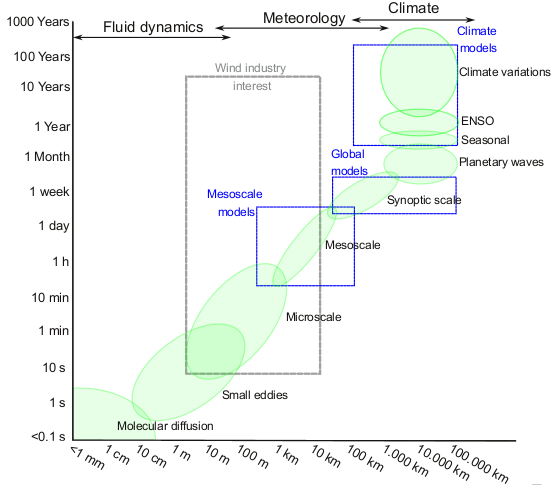
\includegraphics[width=0.7\linewidth]{Imagenes/terraincog}
\caption{Separación de escalas en simulación de mecánica de fluidos.}
\label{fig:terraincog}
\end{figure}


\section{ARW-WRF}
\subsection{Generalidades}
El modelo ARW-WRF (Advanced Research WRF) es un modelo no hidrostático que resuelve el sistema de ecuaciones para flujo compresible en su forma conservativa y utilizando una coordenada vertical de masa (o de presión hidrostática). Su coordenada vertical está definida como:
\begin{equation}
\eta = \frac{p_{dh}-p_{dht}}{\mu_d}
\end{equation}
Donde $p_{dh}$ corresponde a la componente hidrostática de la presión del aire seco, y:
\begin{equation}
\mu_d = p_{dhs} - p_{dht}
\end{equation}
es la masa de aire seco para una columna. En estas ecuaciones los subíndices $t$ y $s$ corresponden a los límites superior (top) e inferior (surface) del dominio. Las variables principales que resuelve el modelo son las velocidades covariantes $(u,v,w)$, masa de aire seco, geopotencial, temperatura potencial ($\theta$) y energía cinética turbulenta (TKE) de submalla (SGS). La ecuación de momentum, temperatura potencial, SGS TKE y otros escalares relevantes tienen una forma acoplada con la masa de aire seco, a priori:
\begin{equation}
\partial_t (\mu_d\theta) + \partial_x(\mu_d\mu\theta)+\partial_y(\mu_d\nu\theta)+\partial_\eta (\mu_d\omega\theta) = F
\end{equation}
Donde $F$ es la suma de la mezcla turbulenta junto con otras fuerzas y
\begin{equation}
\omega = d_t\eta
\end{equation}
es la velocidad en la coordenada vertical.

La discretización en el tiempo se realiza a través de un esquema de integración temporal múltiple. Este esquema separa los modos de alta frecuencia (i.e. ondas acústicas y de gravedad) de los modos de baja frecuencia (modo físico). ARW utiliza un esquema RK3 y durante cada paso en el RK, el modo de alta frecuencia que se propaga horizontalmente es integrado a través de un esquema \emph{forward-backward} utilizando un paso de tiempo acústico, que es típicamente un orden de magnitud mas pequeño que el paso físico, mientras que un esquema implícito es utilizado para el modo de alta frecuencia que se propaga de manera vertical.
\subsection{Ecuaciones Resueltas}
\subsection{Discretización Espacial}
\subsection{Discretización Temporal}
\subsection{Aspectos Numéricos}
\subsubsection{Advección}
\subsubsection{Difusión}
\subsubsection{Microfísicas}


\chapter{Caso de Estudio}
\section{Aspectos Generales}
Para este caso, se está interesado en caracterizar el comportamiento del viento en la zona costera de Valparaíso, mas específicamente en el sector de Laguna Verde, lugar donde existe un gran interés a causa de su alto potencial eólico, tal como lo explicita el Explorador Eólico de la Universidad de Chile y cuyo resultado se puede observar en la figura \ref{fig:explorador}.

\begin{figure}[H]
	\centering
	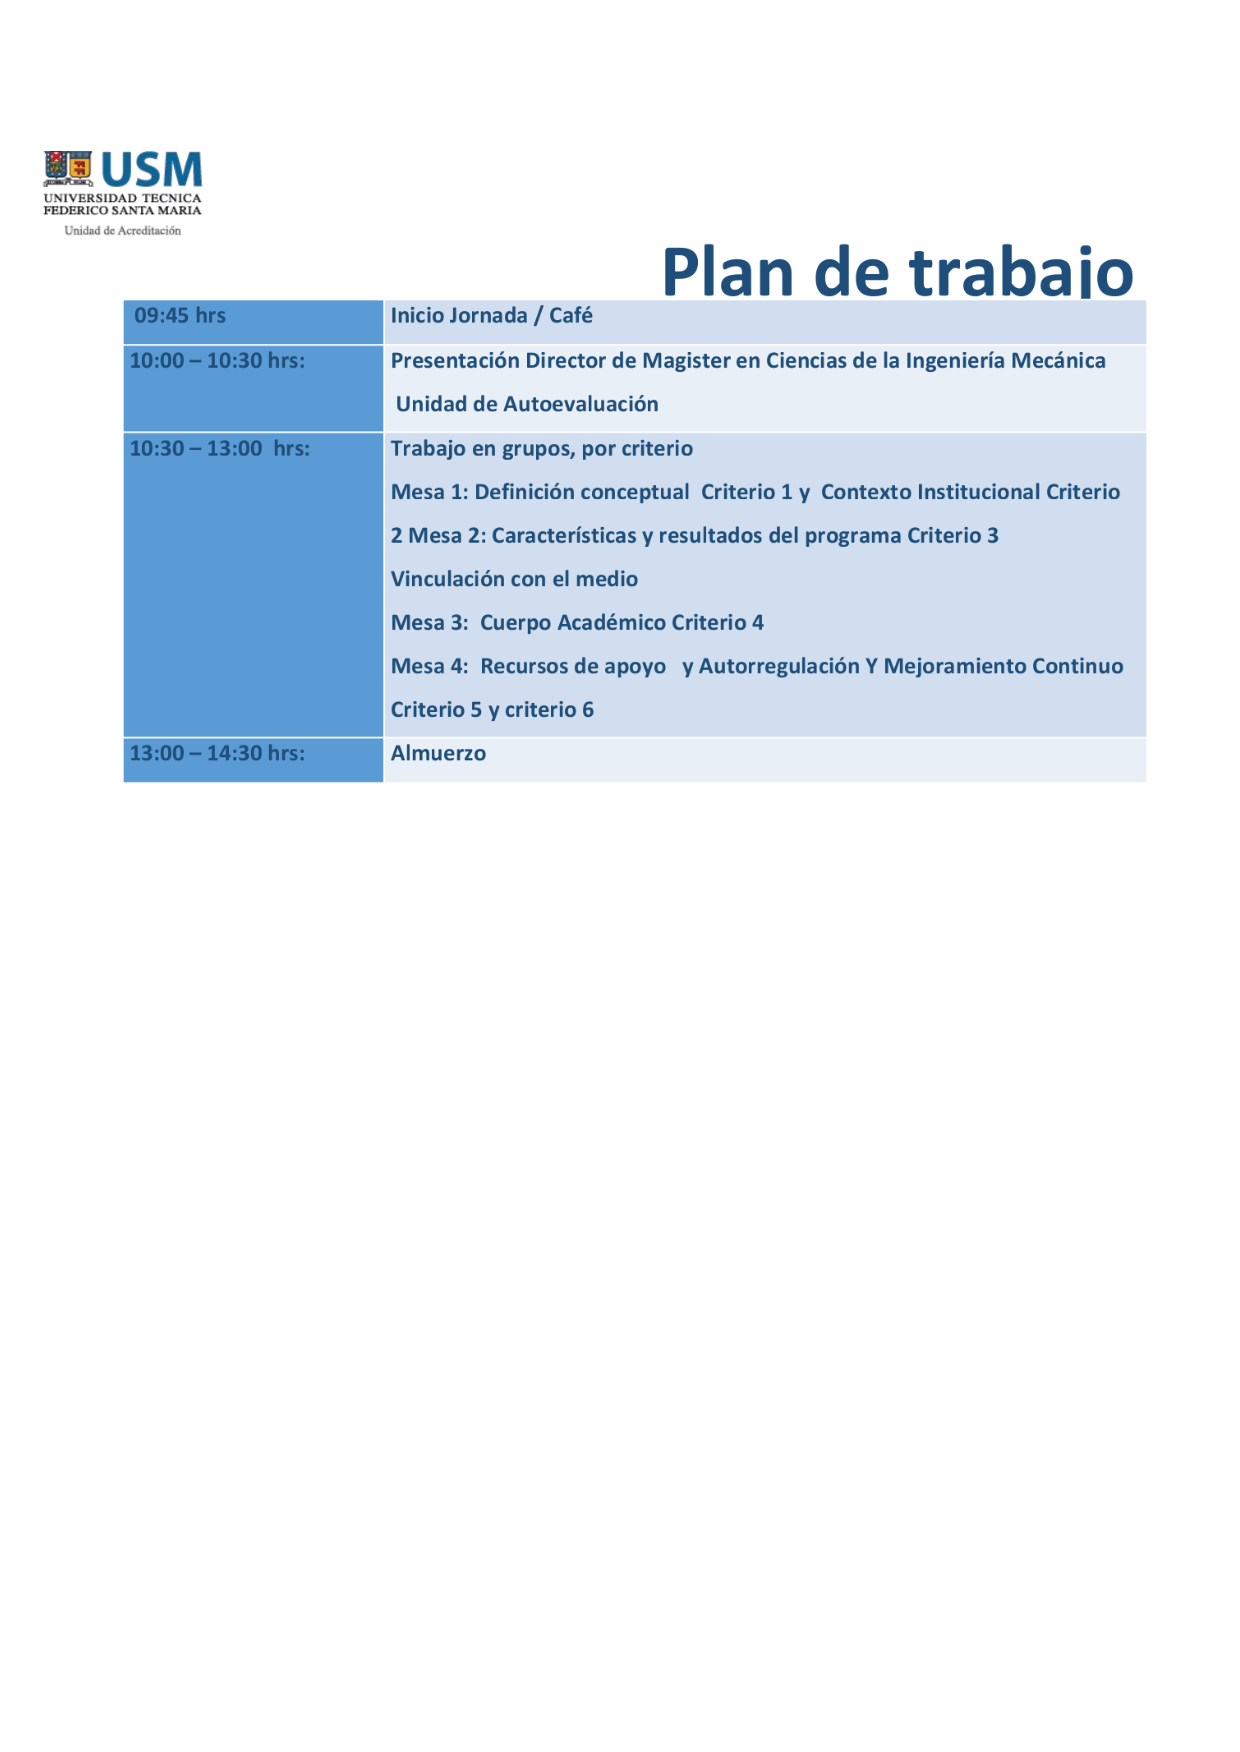
\includegraphics[width=0.9\linewidth,trim={5.4cm 2cm 15cm 5.5cm},clip]{Imagenes/explorador}
	\caption{Información del Explorador Eólico para la zona de interés.}
	\label{fig:explorador}
\end{figure}

Los datos de la figura \ref{fig:explorador} corresponde a un promedio anual para la magnitud de la velocidad en cada punto de la malla numérica. Esta malla tiene una resolución de 1 [km], la cual, si bien permite obtener información relevante acerca de zonas con alto potencial eólico, es ineficiente para capturar el comportamiento del flujo en el terreno complejo. Es por esto, que es relevante afinar la simulaciones aplicando técnicas modernas y apuntar a una mejor calidad para la caracterización eólica de una zona.

La simulación de la que trata este informe se realiza en un día standart del mes de Enero del año 2010. El día de simulación se escogió, por una parte, por las facilidades para obtener las condiciones de contorno provenientes de otros modelos y por otro, por que en verano existe un comportamiento mas energético del viento.
\section{Resolución Espacial}
Se discretiza espacialmente la zona en 6 dominios colocados de forma telescópica y centrados en el punto de coordenadas (-33.097344, -71730552) que corresponde a la costa de Punta Curaimilla.

Como el objetivo principal es obtener una malla fina con resolución de 50 [m], a la malla mas gruesa se le asigna un $\Delta x = \Delta y = 12150$ [m] y cada malla se va afinando en un factor de 3 su resolución. La resolución de malla mas gruesa es electa debido a su compatibilidad con la interpolación de las condiciones de borde del modelo global.

La distribución de las mallas y su proyección sobre la tierra se pueden observar en las figuras \ref{fig:0102}, \ref{fig:0203}, \ref{fig:0304}, \ref{fig:0405} y \ref{fig:0506}.

\begin{figure}[H]
	\centering
	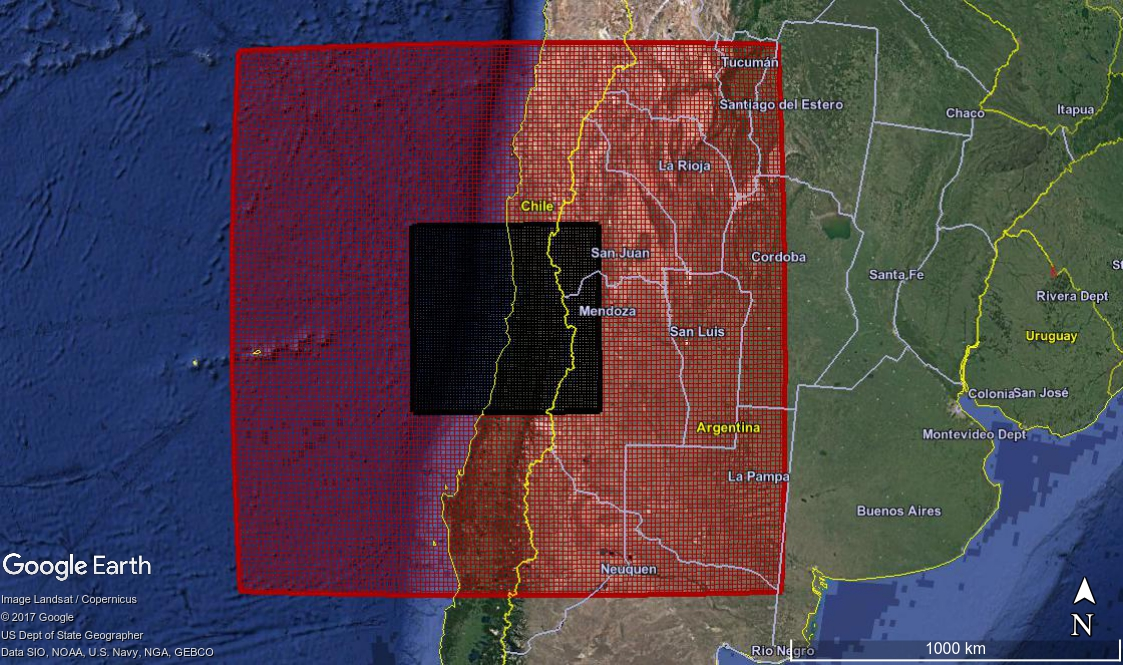
\includegraphics[width=0.95\linewidth]{Imagenes/d06d05}
	\caption{Dominios de las mallas exteriores d01 y d02.}
	\label{fig:0102}
\end{figure}

\begin{figure}[H]
	\centering
	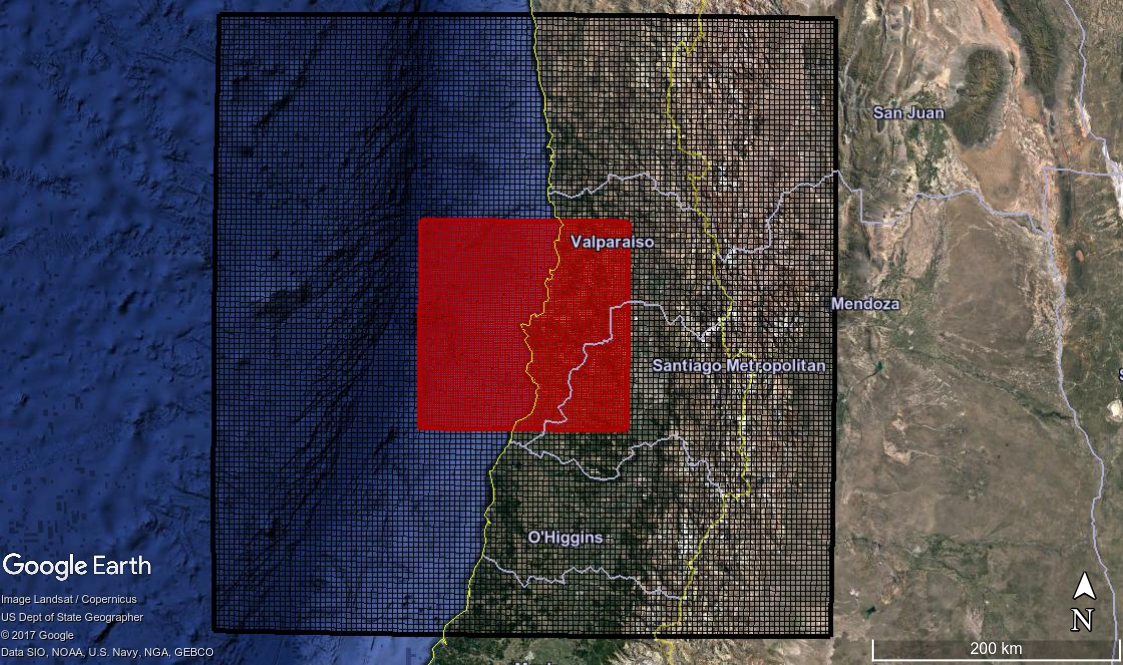
\includegraphics[width=0.95\linewidth]{Imagenes/d05d04}
	\caption{Dominios d02 y d03.}
	\label{fig:0203}
\end{figure}

\begin{figure}[H]
	\centering
	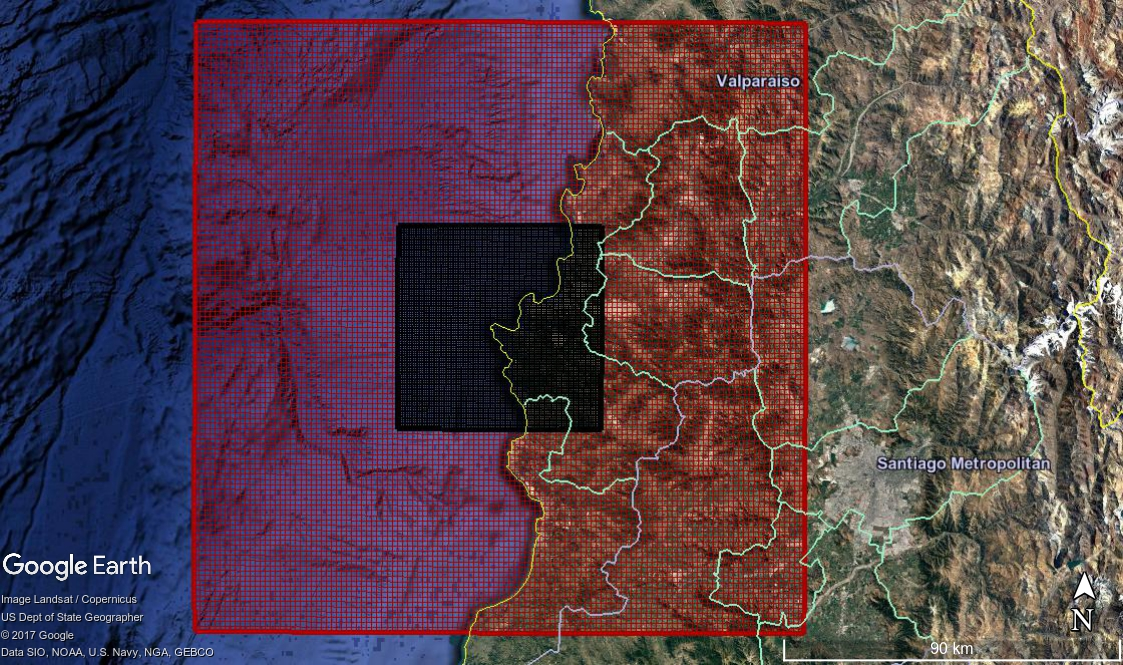
\includegraphics[width=0.95\linewidth]{Imagenes/d04d03}
	\caption{Dominios d03 y d04 (LES).}
	\label{fig:0304}
\end{figure}

\begin{figure}[H]
	\centering
	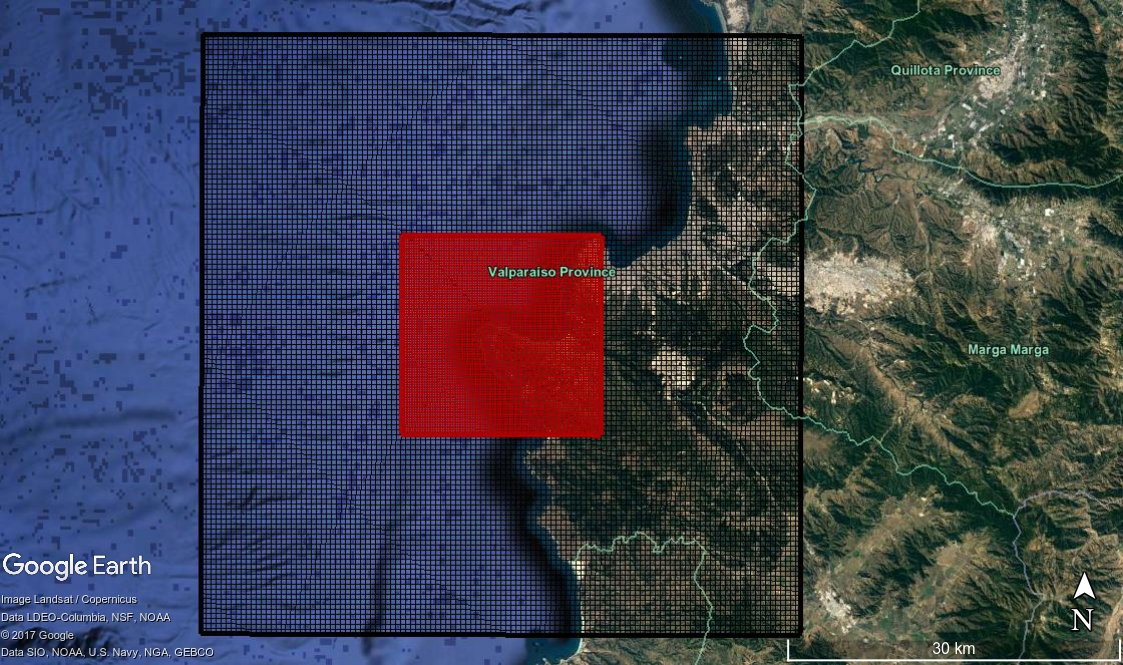
\includegraphics[width=0.95\linewidth]{Imagenes/d03d02}
	\caption{Dominios d04 (LES) y d05 (LES).}
	\label{fig:0405}
\end{figure}

\begin{figure}[H]
	\centering
	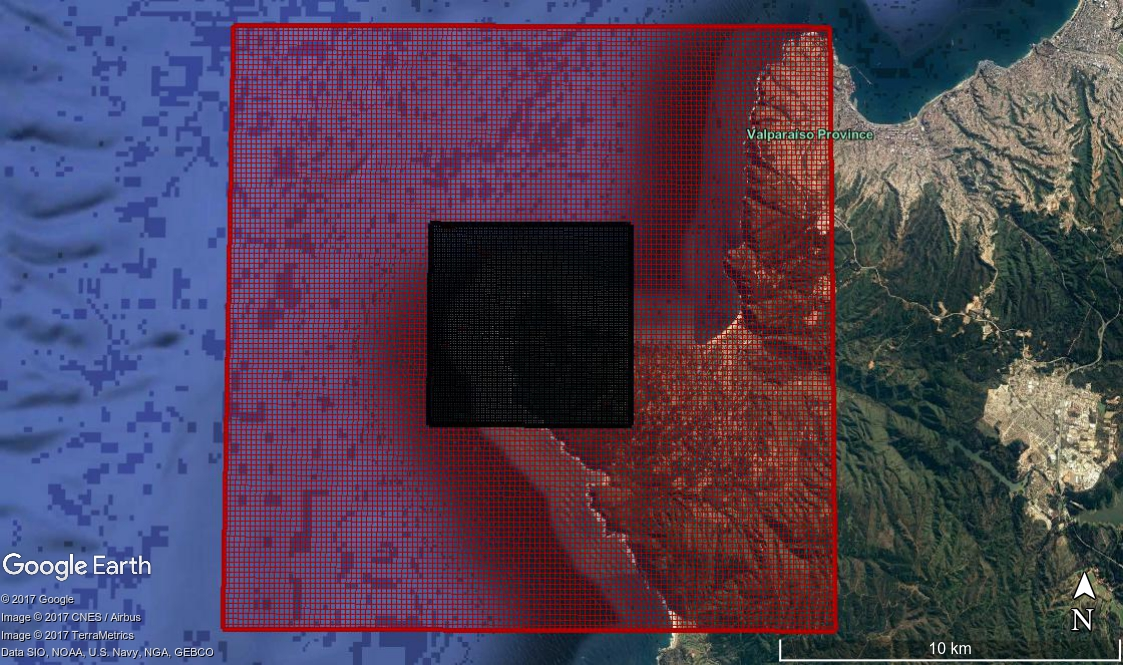
\includegraphics[width=0.95\linewidth]{Imagenes/d02d01}
	\caption{Dominios mas finos d05 (LES) y d06 (LES).}
	\label{fig:0506}
\end{figure}
Cada malla consta de $121\times 121$ nodos en el sentido horizontal y 47 nodos en sentido vertical. Existe un refinamiento de la malla en la cercanía a la superficie de modo de tener los 10 primeros niveles dentro de los primeros 300 [m] de atmósfera.
\section{Resolución Temporal}
Para la simulación se utiliza un paso de tiempo físico constante. Para no tener problemas de inestabilidades y que el modelo diverja, se opta por una relación empírica conservadora que es parte de las buenas prácticas en el uso del WRF. Se utiliza:
\begin{equation}
\Delta t \approx \Delta x
\end{equation}
Donde $\Delta x$ tiene unidades de [km]. Luego, el paso de tiempo para el dominio mas grande será $\Delta x=12$ [s] y este valor va reduciéndose 1/3 en cada dominio anidado. Utilizando este valor no se presentaron problemas en el desarrollo de las iteraciones.
\section{Condiciones de Borde}
Para inicializar el modelo y para proveer de información en los contornos cada 6 horas, se utilizan los datos de los análisis operacionales provenientes del modelo global GFS con resolución de $0.5^\circ$ ($\approx 55.6$ [km])

Por otra parte, como el dominio mas grande a simular cae dentro de lo que es una simulación de mesoescala y tomando en consideración las proyecciones debido a la curvatura de la tierra para esta zona en particular, se decide fijar la condición de borde superior para la coordenada vertical de presión a $p_{dht} = 5000$ [kPa] siguiendo la recomendación del manual del programa.
\section{Información del Terreno}
Debido a que los últimos 3 dominios son de 450, 150 y 50 [m] respectivamente en sus tamaños de malla, es necesario proveer al modelo información superficial de alta resolución. Para la topografía se utilizan los datos de la operación satelital SRTM de la NASA que tienen resolución de 3 segundos de arco. Para las propiedades de la superficie como vegetación, rugosidad, tipo de uso de suelo se utilizan los datos que provienen de los instrumentos satelitales MODIS.
\section{Parametrizaciones}
\begin{table}[h!]
	\caption{Esquemas de Parametrización Utilizados.}\label{tab:esquemas}
	\centering
	\begin{tabular}{lllllll}
		\toprule
		Física 					& d01	&	d02	&	d03	&	d04	&	d05	&	d06 \\
		\midrule
		Micro-físicas		 	& WSM 5-especie&d02&d02&d02&d02&d02  \\
		Cúmulos			 		& -- &d02&d02&d02&d02&d02\\ 
		Capa Superficial	 	& QNSE &d02&d02&d02&d02&d02\\
		PBL				 		& QNSE &d02&d02&d02&d02&d02\\
		Modelo de Suelo 		& 5 capas&d02&d02&d02&d02&d02 	\\
		Radiación Onda Larga	& RRTMG&d02&d02&d02&d02&d02 \\
		Radiación Onda Corta	& Dudhia&d02&d02&d02&d02&d02 \\
		\bottomrule
	\end{tabular}
\end{table}
\section{Monitoreo de Variables}

\chapter{Resultados}
A continuación se muestran los resultados obtenidos de la simulación presentada en la sección anterior. En general, por cada archivo de salida de datos (cada 15 minutos en este caso), se obtienen valores de velocidad, presión, temperatura, humedad, TKE, flujos superficiales, entre otras cantidades que utiliza el modelo en cada punto de la malla desplazada. Sin embargo acá no se presentan tantos datos. La muestra de datos se restringe entonces a mostrar de manera cuantitativa el comportamiento dinámico del flujo en la capa límite del dominio mas fino.
\section{Series de Tiempo}
A continuación se presentan algunos resultados representativos de las series de tiempo obtenidas con la simulación. Se muestran los datos para la magnitud de la velocidad y para la dirección del viento.

\begin{figure}[H]
	\centering
	\includegraphics[width=0.69\linewidth,page=11,trim={3cm 6cm 4cm 8cm},clip]{Imagenes/u_ts}
	%\vspace{-5mm} 
	\caption{Rapidez del viento para $\eta_l=6, z_l=123.349$ [m]}
	\label{ts_rap}
\end{figure}

\begin{figure}[H]
	\centering
	\includegraphics[width=0.77\linewidth,page=12,trim={2cm 7cm 3cm 8cm},clip]{Imagenes/u_ts}
	%\vspace{-5mm} 
	\caption{Ángulo del viento para $\eta_l=6, z_l=123.349$ [m]}
	\label{ts_ang}
\end{figure}

Es importante destacar la alta variabilidad de las variables dentro de las primeras tres horas de simulación. Esto se deben al \emph{spin-up} del modelo. La turbulencia tarda su tiempo en poder desarrollarse y por lo tanto los valores obtenidos en este rango de tiempo se omiten para los futuros resultados ya que contaminan la solución.
\section{Campos de Velocidad}
A continuación se presentan las figuras obtenidas para la velocidad con los datos resultados de la simulación. Se hace énfasis en dos análisis: la rapidez del viento cercano a la superficie, que permite describir la interacción con el terreno complejo, y los promedios de velocidad horizontal en los niveles verticales mas cercanos a la superficie que exhiben el potencial eólico de cada elemento de la malla.
\subsection{Rapidez Instantánea a 10 [m]}
De los resultados de la velocidad, se interpola a través de la ley logarítmica para encontrar la magnitud de la velocidad a 10 [m] sobre la superficie. Las figuras siguientes permiten caracterizar el comportamiento del aire en el terreno complejo, identificando zonas de recirculación.
\newcommand{\velins}[2]{
	\begin{figure}[H]
		\centering
		\includegraphics[width=0.69\linewidth,page=#1,trim={2cm 5cm 1cm 4.5cm},clip]{Imagenes/rapidez_ins_10m}
		%\vspace{-5mm} 
		\caption{Rapidez horizontal a 10 [m] simulada a las #2}
		\label{rap_10m_#2}
	\end{figure}
}
\velins{1}{12:00:00}
\velins{2}{12:15:00}
\velins{3}{12:30:00}
\velins{4}{12:45:00}%
\velins{5}{13:00:00}
\velins{6}{13:15:00}
\velins{7}{13:30:00}
\velins{8}{13:45:00}%
\velins{9}{14:00:00}
\velins{10}{14:15:00}
\velins{11}{14:30:00}
\velins{12}{14:45:00}%
\velins{13}{15:00:00}
\velins{14}{15:15:00}
\velins{15}{15:30:00}
\velins{16}{15:45:00}%
\velins{17}{16:00:00}
\velins{18}{16:15:00}
\velins{19}{16:30:00}
\velins{20}{16:45:00}%
\velins{21}{17:00:00}
\velins{22}{17:15:00}
\velins{23}{17:30:00}
\velins{24}{17:45:00}%
\velins{25}{17:00:00}
\velins{26}{18:15:00}
\velins{27}{18:30:00}
\velins{28}{18:45:00}%
\velins{29}{18:00:00}
\velins{30}{19:15:00}
\velins{31}{19:30:00}
\velins{32}{19:45:00}%
\velins{33}{19:00:00}
\velins{34}{20:15:00}
\velins{35}{20:30:00}
\velins{36}{20:45:00}%
\velins{37}{21:00:00}
\subsection{Velocidad Media}
Se promedian temporalmente los valores obtenidos en cada punto de malla, en cada nivel de la coordenada vertical.

A continuación se presentan los resultados para los primeros 10 niveles (relevantes para aplicaciones eólicas) y se detalla la altura media en metros a la cual se realizó la simulación.
\newcommand{\velmed}[2]{
	\begin{figure}[H]
		\centering
		\includegraphics[width=0.69\linewidth,page=#1,trim={2cm 5cm 1cm 4.5cm},clip]{Imagenes/rapidez_media}
		%\vspace{-5mm} 
		\caption{Rapidez media $\eta_l = #1$. $z_l = #2$ [m]}
		\label{rap_med_#1}
	\end{figure}
}
\velmed{1}{8.20464}
\velmed{2}{24.6166}
\velmed{3}{38.9816}
\velmed{4}{51.2991}
\velmed{5}{82.144}
\velmed{6}{123.349}
\velmed{7}{164.752}
\velmed{8}{218.859}
\velmed{9}{277.528}
\velmed{10}{345.167}
\section{Perfiles de Velocidad}
Las siguiente figuras muestran el perfil de viento medio para las cuatro ubicaciones mencionadas anteriormente.

\newcommand{\velprofile}[2]{
	\begin{figure}[H]
		\centering
		\includegraphics[width=0.7\linewidth,page=#1,trim={2cm 6cm 2cm 7.6cm},clip]{Imagenes/perfil_medio}
		%\vspace{-5mm} 
		\caption{Perfil de viento para #2.}
		\label{rap_perfil_#1}
	\end{figure}
}
\velprofile{1}{(-33.103,-71.716)}
\velprofile{3}{(-33.115,-71.708)}
\velprofile{5}{(-33.110,-71.730)}
\velprofile{7}{(-33.104,-71.704)}
\section{Espectro de Energía}
Para cada serie de tiempo obtenida en el punto de monitoreo, se realiza un análisis espectral a modo de revisar su distribución en el espacio de frecuencias.

Si bien en LES es necesario descomponer en el espacio de números de onda la señal de velocidad, se puede hacer la analogía con el espacio de frecuencias usando la hipótesis de Taylor considerando una turbulencia moderada.

A continuación se presentan los espectros para los primeros 15 niveles de la coordenada vertical. Como referencia también se grafica la ley de los $-5/3$.
\newcommand{\spectrafig}[1]{
\begin{figure}[H]
	\centering
	\includegraphics[width=0.66\linewidth,page=#1,trim={0cm 0cm 0cm 1.4cm},clip]{Imagenes/spectra}
	\vspace{-5mm} 
	\caption{Espectro de velocidad horizontal para $\eta_l = #1$}
	\label{spectra_#1}
\end{figure}
}
\spectrafig{1}
\spectrafig{2}
\spectrafig{3}
\spectrafig{4}
\spectrafig{5}
\spectrafig{6}
\spectrafig{7}
\spectrafig{8}
\spectrafig{9}
\spectrafig{10}
\spectrafig{11}
\spectrafig{12}
\spectrafig{13}
\spectrafig{14}
\spectrafig{15}



\chapter{Análisis y Conclusiones}
Del análisis de los resultados obtenidos se extraen la siguientes conclusiones:
\begin{itemize*}
	\item Debido a la simulación lograda con las bases de datos de alta resolución y aplicando LES para la turbulencia, se puede ver claramente el comportamiento del flujo sobre el terreno complejo de Punta Curaumilla. El explorador eólico reconoce toda la zona como una zona de alto potencial eólico, sin embargo, un mejor análisis permite ver la formación de zonas de recirculación y las zonas localizadas de vientos horizontales fuertes.
	\item Con respecto a los perfiles de velocidad, esto cumplen lo esperado en su forma. Como el día es de Enero, no se espera tener perfiles con formas fuera de lo común, sin embargo la comparación entre los 4 puntos permite comprobar las estadísticas obtenidas en los otros resultados.
	\item Los valores medios obtenidos para cada nivel permiten el reconocimiento de dos zonas que destacan por su alto potencial eólico y que vendrían a ser buenos candidatos para futuros proyectos eólicos. Una de estas es la costa central del dominio y la otra es la zona aguasabajo de la colina simulada.
	\item El espectro de energía obtenido de las mediciones continuas para la velocidad horizontal tiene una forma concordante con la teoría. Si bien la zona inercial no cumple a cabalidad la ley de los -5/3, esto es de esperar debido a que la turbulencia en la capa límite atmosférica está lejos de ser homogénea e isotrópica. Se puede apreciar que a medida que se aumenta en los niveles de la coordenada vertical, el espectro poco a poco va aumentando su pendiente, acercándose a los -5/3. Esto se explica debido a que lejos de la superficie ya no existen direcciones preferentes para la turbulencia y está comienza su transición a la isotropía.
\end{itemize*}
\section{Trabajo Futuro}
Para el caso de estudio revisado en este informe y su respectiva simulación queda por realizar las siguientes tareas:
\begin{itemize*}
	\item Expandir las simulaciones a una mayor ventana temporal, utilizando un mejor recurso computacional para aprovechar la paralelización del código y así obtener mejores estadísticos de la zona.
	\item Hacer un análisis de sensibilidad a los distintos factores externos de la simulación: condiciones de borde, esquemas de parametrización de la microfísica, cambiar modelos de advección-difusión, etc.
	\item Simular utilizando un dominio computacional mas grande, es decir, aumentar el número de nodos en la dirección horizontal, para que de esta forma sea representativo realizar un análisis espectral en el espacio de números de onda y obtener directamente el espectro de energía turbulenta.
	\item La utilización y comparación con otros modelos de submalla. Específicamente revisar el comportamiento con un modelo de Smagorinsky 3D y otros modelos anisotrópicos.
	\item Validar las simulaciones realizadas con mediciones reales. Estas se esperan que estén operativas en algún momento año 2018.
\end{itemize*}

%%
\appendix
%%%% Cap'itulos incluidos despues del comando \appendix aparecen como ap'endices
%%%% de la tesis.

%%Apendice A
%
\chapter{Titulo Apendice A}

%%Apendice B
%
\chapter{Titulo Apendice B}

%

%%% Incluir la bibliograf'ia. Mirar el archivo "biblio.bib" para m'as detales
%%% y un ejemplo.
%

\nocite{*}     %incluir en la bibliografia articulos no citados
\bibliography{Bibliografia/biblio}

\end{document}
